%%%%%%%%%%%%%%%%%%%%%%%%%%%%%%%%%%%%%%%%%
% Programming/Coding Assignment
% LaTeX Template
%
% This template has been downloaded from:
% http://www.latextemplates.com
%
% Original author:
% Ted Pavlic (http://www.tedpavlic.com)
%
% Note:
% The \lipsum[#] commands throughout this template generate dummy text
% to fill the template out. These commands should all be removed when 
% writing assignment content.
%
% This template uses a Perl script as an example snippet of code, most other
% languages are also usable. Configure them in the "CODE INCLUSION 
% CONFIGURATION" section.
%
%%%%%%%%%%%%%%%%%%%%%%%%%%%%%%%%%%%%%%%%%

%----------------------------------------------------------------------------------------
%	PACKAGES AND OTHER DOCUMENT CONFIGURATIONS
%----------------------------------------------------------------------------------------

\documentclass{article}

\usepackage{fancyhdr} % Required for custom headers
\usepackage{lastpage} % Required to determine the last page for the footer
\usepackage{extramarks} % Required for headers and footers
\usepackage[usenames,dvipsnames]{color} % Required for custom colors
\usepackage{graphicx} % Required to insert images
\usepackage{subcaption}
\usepackage{listings} % Required for insertion of code
\usepackage{courier} % Required for the courier font
\usepackage{lipsum} % Used for inserting dummy 'Lorem ipsum' text into the template

% Margins
\topmargin=-0.45in
\evensidemargin=0in
\oddsidemargin=0in
\textwidth=6.5in
\textheight=9.0in
\headsep=0.25in

\linespread{1.1} % Line spacing

% Set up the header and footer
\pagestyle{fancy}
\lhead{\hmwkAuthorName} % Top left header
\chead{\hmwkClass\ (\hmwkClassTime): \hmwkTitle} % Top center head
%\rhead{\firstxmark} % Top right header
\lfoot{\lastxmark} % Bottom left footer
\cfoot{} % Bottom center footer
\rfoot{Page\ \thepage\ of\ \protect\pageref{LastPage}} % Bottom right footer
\renewcommand\headrulewidth{0.4pt} % Size of the header rule
\renewcommand\footrulewidth{0.4pt} % Size of the footer rule

\setlength\parindent{0pt} % Removes all indentation from paragraphs

%----------------------------------------------------------------------------------------
%	CODE INCLUSION CONFIGURATION
%----------------------------------------------------------------------------------------

\definecolor{MyDarkGreen}{rgb}{0.0,0.4,0.0} % This is the color used for comments
\lstloadlanguages{Perl} % Load Perl syntax for listings, for a list of other languages supported see: ftp://ftp.tex.ac.uk/tex-archive/macros/latex/contrib/listings/listings.pdf
\lstset{language=Perl, % Use Perl in this example
        frame=single, % Single frame around code
        basicstyle=\small\ttfamily, % Use small true type font
        keywordstyle=[1]\color{Blue}\bf, % Perl functions bold and blue
        keywordstyle=[2]\color{Purple}, % Perl function arguments purple
        keywordstyle=[3]\color{Blue}\underbar, % Custom functions underlined and blue
        identifierstyle=, % Nothing special about identifiers                                         
        commentstyle=\usefont{T1}{pcr}{m}{sl}\color{MyDarkGreen}\small, % Comments small dark green courier font
        stringstyle=\color{Purple}, % Strings are purple
        showstringspaces=false, % Don't put marks in string spaces
        tabsize=5, % 5 spaces per tab
        %
        % Put standard Perl functions not included in the default language here
        morekeywords={rand},
        %
        % Put Perl function parameters here
        morekeywords=[2]{on, off, interp},
        %
        % Put user defined functions here
        morekeywords=[3]{test},
       	%
        morecomment=[l][\color{Blue}]{...}, % Line continuation (...) like blue comment
        numbers=left, % Line numbers on left
        firstnumber=1, % Line numbers start with line 1
        numberstyle=\tiny\color{Blue}, % Line numbers are blue and small
        stepnumber=5 % Line numbers go in steps of 5
}

% Creates a new command to include a perl script, the first parameter is the filename of the script (without .pl), the second parameter is the caption
\newcommand{\perlscript}[2]{
\begin{itemize}
\item[]\lstinputlisting[caption=#2,label=#1]{#1.pl}
\end{itemize}
}

%----------------------------------------------------------------------------------------
%	DOCUMENT STRUCTURE COMMANDS
%	Skip this unless you know what you're doing
%----------------------------------------------------------------------------------------

% Header and footer for when a page split occurs within a problem environment
\newcommand{\enterProblemHeader}[1]{
%\nobreak\extramarks{#1}{#1 continued on next page\ldots}\nobreak
%\nobreak\extramarks{#1 (continued)}{#1 continued on next page\ldots}\nobreak
}

% Header and footer for when a page split occurs between problem environments
\newcommand{\exitProblemHeader}[1]{
%\nobreak\extramarks{#1 (continued)}{#1 continued on next page\ldots}\nobreak
%\nobreak\extramarks{#1}{}\nobreak
}

\setcounter{secnumdepth}{0} % Removes default section numbers
\newcounter{homeworkProblemCounter} % Creates a counter to keep track of the number of problems
\setcounter{homeworkProblemCounter}{0}

\newcommand{\homeworkProblemName}{}
\newenvironment{homeworkProblem}[1][Part \arabic{homeworkProblemCounter}]{ % Makes a new environment called homeworkProblem which takes 1 argument (custom name) but the default is "Problem #"
\stepcounter{homeworkProblemCounter} % Increase counter for number of problems
\renewcommand{\homeworkProblemName}{#1} % Assign \homeworkProblemName the name of the problem
\section{\homeworkProblemName} % Make a section in the document with the custom problem count
\enterProblemHeader{\homeworkProblemName} % Header and footer within the environment
}{
\exitProblemHeader{\homeworkProblemName} % Header and footer after the environment
}

\newcommand{\problemAnswer}[1]{ % Defines the problem answer command with the content as the only argument
\noindent\framebox[\columnwidth][c]{\begin{minipage}{0.98\columnwidth}#1\end{minipage}} % Makes the box around the problem answer and puts the content inside
}

\newcommand{\homeworkSectionName}{}
\newenvironment{homeworkSection}[1]{ % New environment for sections within homework problems, takes 1 argument - the name of the section
\renewcommand{\homeworkSectionName}{#1} % Assign \homeworkSectionName to the name of the section from the environment argument
\subsection{\homeworkSectionName} % Make a subsection with the custom name of the subsection
\enterProblemHeader{\homeworkProblemName\ [\homeworkSectionName]} % Header and footer within the environment
}{
\enterProblemHeader{\homeworkProblemName} % Header and footer after the environment
}

%----------------------------------------------------------------------------------------
%	NAME AND CLASS SECTION
%----------------------------------------------------------------------------------------

\newcommand{\hmwkTitle}{Assignment 2 \\ $[Environment]$ py3.6 with random.seed(1)} % Assignment title
\newcommand{\hmwkDueDate}{Sunday,\ Feburary\ 18,\ 2018} % Due date
\newcommand{\hmwkClass}{CSC411} % Course/class
\newcommand{\hmwkClassTime}{L0101} % Class/lecture time
\newcommand{\hmwkAuthorName}{Yi-Hsun Lee, Yufeng Li} % Your name

%----------------------------------------------------------------------------------------
%	TITLE PAGE
%----------------------------------------------------------------------------------------

\title{
\vspace{2in}
\textmd{\textbf{\hmwkClass:\ \hmwkTitle}}\\
\normalsize\vspace{0.1in}\small{Due\ on\ \hmwkDueDate}\\
\vspace{0.1in}
\vspace{3in}
}

\author{\textbf{\hmwkAuthorName}}
%\date{} % Insert date here if you want it to appear below your name

%----------------------------------------------------------------------------------------

\begin{document}

\maketitle
\clearpage
%----------------------------------------------------------------------------------------
%	PROBLEM 1
%----------------------------------------------------------------------------------------

% To have just one problem per page, simply put a \clearpage after each problem

\begin{homeworkProblem}

\noindent \textit{Dataset description}
\\I picked 10 pictures of each digit from MNIST dataset. For every single digit, there are multiple ways to write. For example, people can write 1 in both handwritten and printed style. This provides a more variant collection of digits.



\begin{figure*}[h!]
    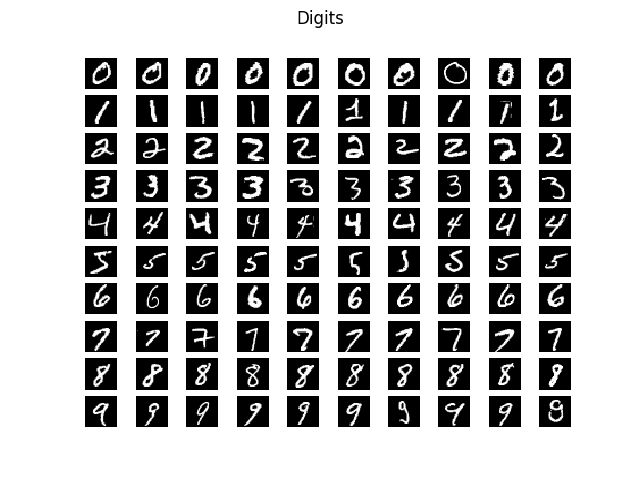
\includegraphics[scale=0.5]{part1.png}
    \caption{A selection of 10 picture of each digit from the MNIST}
    \label{fig:part1}
\end{figure*}


\end{homeworkProblem}
\clearpage
%----------------------------------------------------------------------------------------
%	PROBLEM 2
%----------------------------------------------------------------------------------------

\begin{homeworkProblem}
\noindent \textit{Construct Neural network}
\begin{verbatim}
    def softmax(y):
        return exp(y) / tile(sum(exp(y), 0), (len(y), 1))
    def forward(x, w):
        L0 = dot(w.T, x)
        output = softmax(L0)
        return output
\end{verbatim}
Suppose n is number of pictures, taking bias into account, x is 785*n input array, y is 10*n label array, w is 785*10 weight array.
\end{homeworkProblem}
\clearpage
%----------------------------------------------------------------------------------------
%	PROBLEM 3
%----------------------------------------------------------------------------------------

\begin{homeworkProblem}
\noindent \textit{Construct Gradient Descend}

\begin{figure*}[h!]
    \includegraphics[scale=0.5]{part3.png}
    \caption{Gradient function justification}
    \label{fig:part1}
\end{figure*}
\\Below is the vectorized code for gradient function.
\begin{verbatim}
    def df(w, x, y):
        output = forward(x, w)
        return dot(x, (output - y).T)
\end{verbatim}
\\I calculated the finite difference's output and my gradient function's output and compare the average error. Using the code above.
\begin{verbatim}
    def finite_difference(x, y, theta, h):
        origin_t = f(theta, x, y)
        theta = theta + np.full((theta.shape[0], theta.shape[1]), h)
        after_t = f(theta, x, y)
        finite_diff = (after_t - origin_t) / h
        total_error = sum(finite_diff - df(theta, x, y))
        return abs(total_error) / (785 * 10 * 1.0)
    np.random.seed(1)
    W0 = np.random.randn(785, 10) / sqrt(785)
    x, y = generate_x_y('train', 200)
    print(finite_difference(x, y, W0, 1e-3))
\end{verbatim}
Which has the output
\begin{verbatim}
    finite_difference:2.21852260554e-15
\end{verbatim}
This proves my gradient is indeed the true gradient of the cost function. Since the avg. error is rather insignificant.
\end{homeworkProblem}
\clearpage

%----------------------------------------------------------------------------------------
%	PROBLEM 4
%----------------------------------------------------------------------------------------

\begin{homeworkProblem}
\noindent \textit{Train the neural network using SDG}
\\Specifically, I like to show how I find the learning rate and how I initialized the weight. 
\\I tried alpha in range of (0, 1e-1, 1e-2)
and I get a plot of alpha against accuracy of test samples. See Figure 3 below. Clearly, 1e-2 was a good choice since it has the highest accuracy.
\begin{verbatim}
    alpha = np.arange(0, 1e-1, 1e-2)
    alpha_p = []
    for a in alpha:
        W = sgd(x, y, W0, df, a, 2000)
        alpha_p.append(testing(W))
\end{verbatim}
\begin{figure*}[h!]
    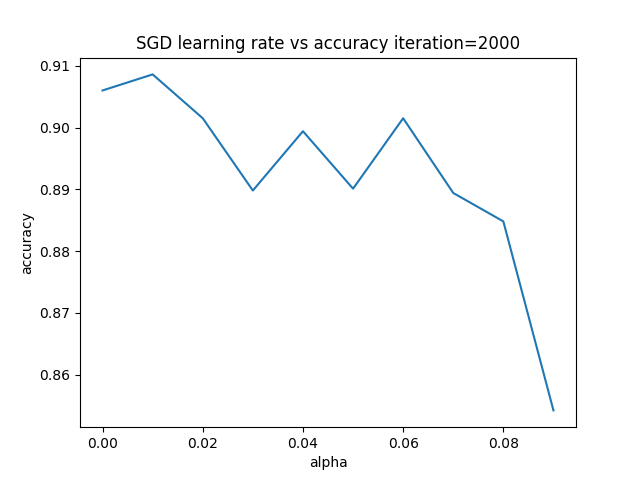
\includegraphics[scale=1]{SGDaccuracy.png}
    \caption{SGD alpha vs accuracy}
    \label{fig:sdg}
\end{figure*}
\\I initialized my weight using Gaussian and use np.random.randn() to generate weight with shape of (785,10) and the variance is 1/size_{in}.
\begin{verbatim}
    #Code for generating W0:
    np.random.randn(785, 10) / sqrt(785)
\end{verbatim}
\clearpage
And I get the following weights below:
\begin{figure*}[!ht]
\begin{subfigure}{.35\textwidth}
  \centering
  
\includegraphics[width=.35\linewidth]{0.png}
  \caption{0's weight}
  \label{fig:1}
\end{subfigure}%
\begin{subfigure}{.35\textwidth}
  \centering
  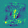
\includegraphics[width=.35\linewidth]{1.png}
  \caption{1's weight}
  \label{fig:2}
\end{subfigure}%
\break
\begin{subfigure}{.35\textwidth}
  \centering
  
\includegraphics[width=.35\linewidth]{2.png}
  \caption{2's weight}
  \label{fig:3}
\end{subfigure}%
\begin{subfigure}{.35\textwidth}
  \centering
  
\includegraphics[width=.35\linewidth]{3.png}
  \caption{3's weight}
  \label{fig:4}
\end{subfigure}%
\break
\begin{subfigure}{.35\textwidth}
  \centering
  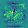
\includegraphics[width=.35\linewidth]{4.png}
  \caption{4's weight}
  \label{fig:5}
\end{subfigure}%
\begin{subfigure}{.35\textwidth}
  \centering
  
\includegraphics[width=.35\linewidth]{5.png}
  \caption{5's weight}
  \label{fig:6}
\end{subfigure}%
\break
\begin{subfigure}{.35\textwidth}
  \centering
  
\includegraphics[width=.35\linewidth]{6.png}
  \caption{6's weight}
  \label{fig:5}
\end{subfigure}%
\begin{subfigure}{.35\textwidth}
  \centering
  
\includegraphics[width=.35\linewidth]{7.png}
  \caption{7's weight}
  \label{fig:6}
\end{subfigure}%
\break
\begin{subfigure}{.35\textwidth}
  \centering
  
\includegraphics[width=.35\linewidth]{8.png}
  \caption{8's weight}
  \label{fig:5}
\end{subfigure}%
\begin{subfigure}{.35\textwidth}
  \centering
  
\includegraphics[width=.35\linewidth]{9.png}
  \caption{9's weight}
  \label{fig:6}
\end{subfigure}%
\end{figure*}
\\Since we uses mini-batch, We should expect it to be noisy since we divide whole batch into mini-batches and update weight each mini-batch.
\clearpage
And here's is the learning curve using SDG:
\begin{figure*}[h!]
    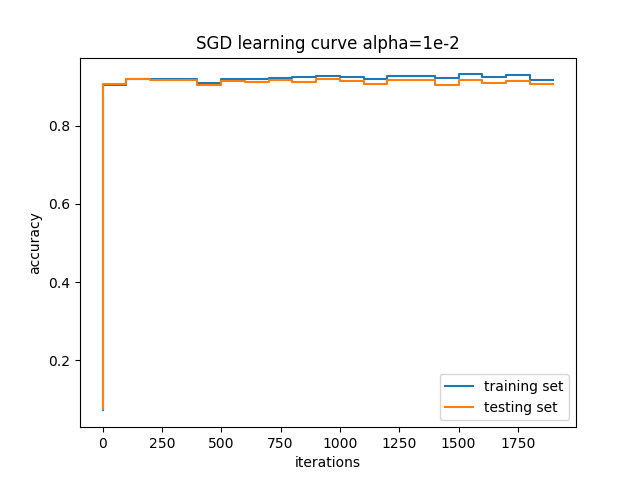
\includegraphics[scale=1]{SGD.png}
    \caption{SGD learning curve}
    \label{fig:sdg}
\end{figure*}
\\Since our training set is large enough so that many variations have taken count into the weight, the testing set's performance is very high at this point compared to training set. However, it starts to fluctuate at 750 iterations and there's no more improvement from there.
\\\textbf{Note}: There's no validating set in mnist\_all.mat file



\end{homeworkProblem}
\clearpage

%----------------------------------------------------------------------------------------

%----------------------------------------------------------------------------------------
%	PROBLEM 5
%----------------------------------------------------------------------------------------


\begin{homeworkProblem}
\noindent \textit{Train the neural network using SDG with momentum}
\\Code I use to do SGD with momentum:
\begin{verbatim}
    def next_batch(x, y, batchSize):
        for i in np.arange(0, x.shape[1], batchSize):
            if (i + batchSize) < x.shape[1]:
                yield (x[:, [i, i + batchSize]], y[:, [i, i + batchSize]])
            else:
                yield (x[:, [i, x.shape[1] - 1]], y[:, [i, y.shape[1] - 1]])
    
    def sgd_momentum(x, y, w, df, alpha, epoch):
        it = 0
        velocity = zeros_like(w)
        while it < epoch:
            x, y = shuffle_input(x, y)
            for (batchX, batchY) in next_batch(x, y, 128):
                velocity = 0.9 * velocity + alpha * df(w, batchX, batchY)
                w -= velocity
            it += 1
        return w
\end{verbatim}
\clearpage
\\And the learning curve using SDG momentum:
\begin{figure*}[h!]
    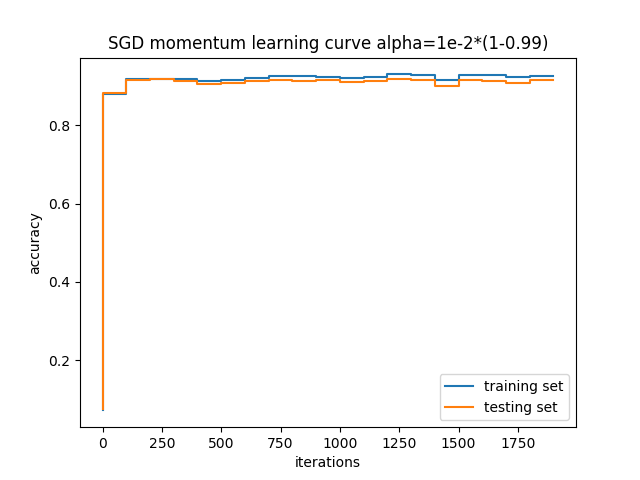
\includegraphics[scale=1]{SGDm.png}
    \caption{SGD with momentum learning curve}
    \label{fig:sdgm}
\end{figure*}
\\We can observe that the performance of testing set starts to fluctuate after 500 iterations and there's no more improvements from there compared to that of 750 iterations in SGD. The reason behind this is because with a smaller amount of iterations, by utilizing momentum, it descends faster, thus a closer approach to perfect weight which leads to the best performance. However, this effect dissipates after more epochs since we have already obtained a good weight and there's no point of accelerating the descend.
\\\textbf{Note}: There's no validating set in mnist\_all.mat file



\end{homeworkProblem}
\clearpage

%----------------------------------------------------------------------------------------

%----------------------------------------------------------------------------------------
%	PROBLEM 6
%----------------------------------------------------------------------------------------


\begin{homeworkProblem}
\noindent \textit{Contour Plot}
\begin{figure*}[h!]
    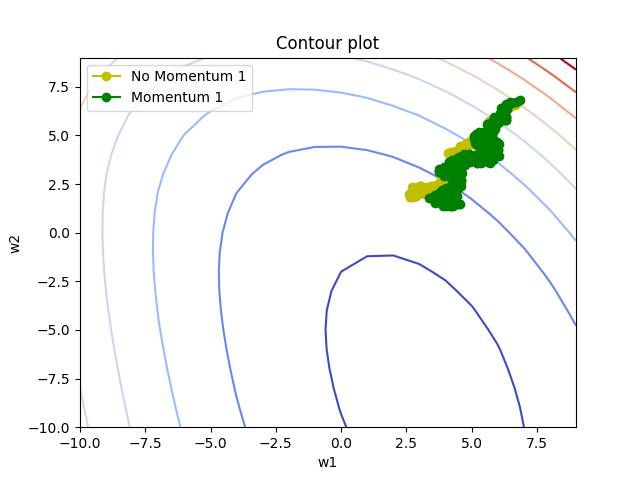
\includegraphics[scale=0.5]{Contour1.png}
    \caption{Contour plot with two trajectories at steeper position}
    \label{fig:cplot}
\end{figure*}
\begin{figure*}[h!]
    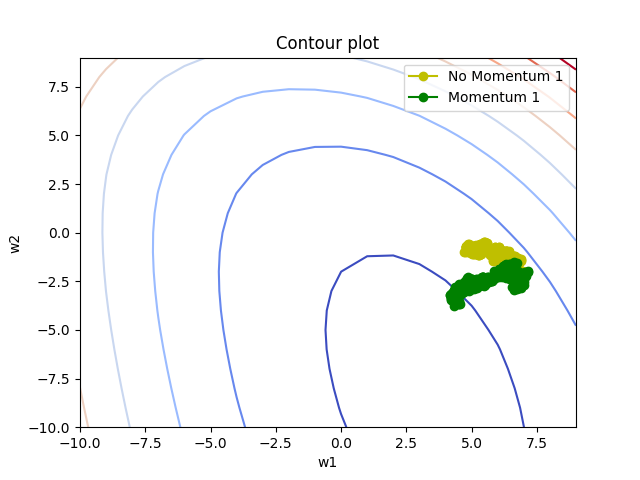
\includegraphics[scale=0.5]{Contour2.png}
    \caption{Contour plot with two trajectories at flatter position}
    \label{fig:cplot}
\end{figure*}
\\As we can see from Figure 8, w1,w2 initialized at flatter position on contour plot,the trajectory of SGD with momentum descend faster than that of without momentum. However, in other scenarios, in Figure 7, I initialized the weights away from optimum and at steeper position in contour plot. Somehow, there's no big difference in both trajectories' descending speed. The reason behind this is that the velocity in momentum will be greater at flat position and smaller at steep position. Since at steeper positions, both momentum and without momentum methods can descend faster.
\\\textbf{Note}: I pick two weights that are in the centre of digits but not right close to each other.




\end{homeworkProblem}
\clearpage

%----------------------------------------------------------------------------------------

%----------------------------------------------------------------------------------------
%	PROBLEM 7
%----------------------------------------------------------------------------------------


\begin{homeworkProblem}
\noindent \textit{Show back propagation faster than update-each-weight method}
\\I construct a new gradient descend function but this time i will update each weight (i.e. not vectorize it). The code is below:
\begin{verbatim}
    def update_every_weight(x, y, w, wi, wj, alpha, output):
        error = output[wj] - y[wj]
        w[wi, wj] -= alpha * np.sum(error * x[wi])


    def gradient_descend(x, y, w, alpha, epoch):
        it = 0
        while it < epoch:
            x, y = shuffle_input(x, y)
            for (batchX, batchY) in next_batch(x, y, 128):
                for wi in range(w.shape[0]):
                    for wj in range(w.shape[1]):
                        output = forward(x, w)
                        update_every_weight(batchX, batchY, w, wi, wj, alpha, output)
            it += 1
        return w
\end{verbatim}
\\I calculate cost function w.r.t. each weight every time using \textbf{\textit{update\_every\_weight}} and update that weight, it follows the not vectorized version of gradient of cost function obtained in \textbf{part3}.
\\I compared it with SGD (i.e. one back propagation method)w.r.t running time using:
\begin{verbatim}
    from timeit import default_timer as timer
    start=timer()
    _=sgd(x, y, W0, df, 1e-2, 10)
    backp_end=timer()-start
    _=gradient_descend(x,y,W0,1e-2,10)
    end=timer()-start
    everyw_end=end-backp_end
\end{verbatim}
And here I got the result:
\begin{verbatim}
    back propagation finished in: 5.358921677048784
    update-every-weight finished in: 1262.9500488219783
    accelerating ratio: 235.67242160506785
\end{verbatim}
Which is approx. power of 3.5 faster than update every weight.

\end{homeworkProblem}
\clearpage

%----------------------------------------------------------------------------------------

%----------------------------------------------------------------------------------------
%	PROBLEM 8
%----------------------------------------------------------------------------------------


\begin{homeworkProblem}
\noindent \textit{Faces Classification with NN\\}

[Part 8 Environment] Using Pytorch without GPU on Windows 10, All images using for datasets were checked with SHA256. \\

First, we try to determine which dimension of the hidden is the best of our dataset: \\

Our first attempt was done without the presence of the validation set, which was a mistake:
\begin{figure*}[h!]
    \begin{center}
    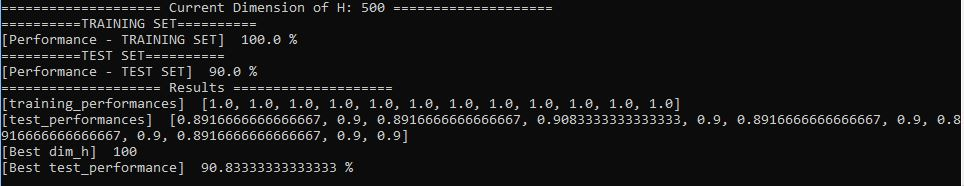
\includegraphics[scale=0.7]{part8-best-dim_h_training_70_testing_20.JPG}
    \caption{First/False Attempt: Training Size = 70, Testing Size = 20, max\_iter=10000}
    \label{fig:part8}
    \end{center}
\end{figure*}
\clearpage
Realizing that we still require the validation set, we decided to take 10 images out of the training set in the first attempt and dedicate those to our validation set:
\begin{figure*}[h!]
    \begin{center}
    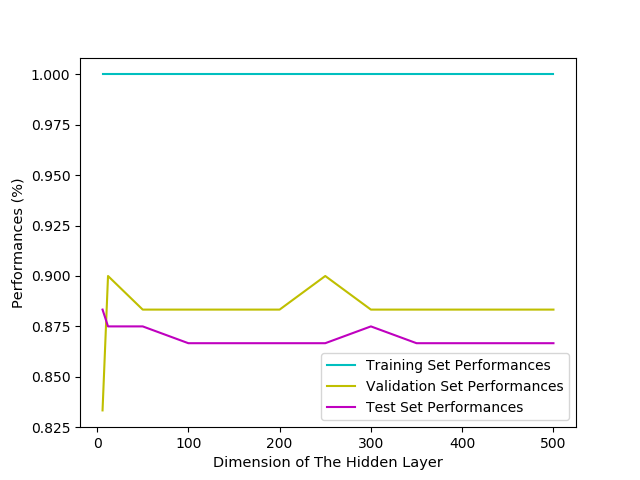
\includegraphics[scale=0.9]{part8-best-dim_h-plot.png}
    \caption{Second/Final Attempt: Training Size = 60, Validating Size = 10, Testing Size = 20, max\_iter=10000}
    \label{fig:part8}
    \end{center}
\end{figure*}

Now we got the best dimension of our hidden layer, which is 12 neurons.
\clearpage

Using the best dim\_h from the results of different trials (dim\_h = 12), we can now get apply this to get our learning curve:
\begin{figure*}[h!]
    \begin{center}
    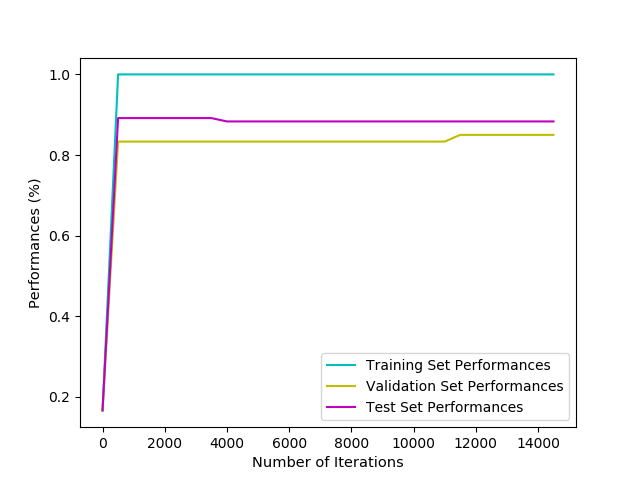
\includegraphics[scale=0.9]{part8-performances-plot.png}
    \caption{Learning Curve: Training Size = 60, Validating Size = 10, Testing Size = 20, dim\_h = 12 (From Previous Figure.)}
    \label{fig:part8}
    \end{center}
\end{figure*}

We now get the best number of iterations we should use to get the best outcome/performance.\\

Note that we can see that our model is slightly over-fitting since the overall performance on the training set is higher than the other two.

\end{homeworkProblem}
\clearpage

%----------------------------------------------------------------------------------------

%----------------------------------------------------------------------------------------
%	PROBLEM 9
%----------------------------------------------------------------------------------------


\begin{homeworkProblem}
\noindent \textit{Weights Visualizations\\}

\begin{figure*}[!ht]
\begin{center}
\begin{subfigure}{.35\textwidth}
  \centering
  
\includegraphics[width=.75\linewidth]{part9-weight_0.png}
  \caption{Lorraine Bracco's weight}
  \label{fig:1}
\end{subfigure}%
\begin{subfigure}{.35\textwidth}
  \centering
  
\includegraphics[width=.75\linewidth]{part9-weight_1.png}
  \caption{Peri Gilpin's weight}
  \label{fig:2}
\end{subfigure}%
\break
\begin{subfigure}{.35\textwidth}
  \centering
  
\includegraphics[width=.75\linewidth]{part9-weight_2.png}
  \caption{Angie Harmon's weight}
  \label{fig:3}
\end{subfigure}%
\begin{subfigure}{.35\textwidth}
  \centering
  
\includegraphics[width=.75\linewidth]{part9-weight_3.png}
  \caption{Alec Baldwin's weight}
  \label{fig:4}
\end{subfigure}%
\break
\begin{subfigure}{.35\textwidth}
  \centering
  
\includegraphics[width=.75\linewidth]{part9-weight_4.png}
  \caption{Bill Hader's weight}
  \label{fig:5}
\end{subfigure}%
\begin{subfigure}{.35\textwidth}
  \centering
  
\includegraphics[width=.75\linewidth]{part9-weight_5.png}
  \caption{Steve Carell's weight}
  \label{fig:6}
\end{subfigure}%
\end{center}
\end{figure*}

\end{homeworkProblem}
\clearpage

%----------------------------------------------------------------------------------------

%----------------------------------------------------------------------------------------
%	PROBLEM 10
%----------------------------------------------------------------------------------------


\begin{homeworkProblem}
\noindent \textit{Transfer Learning with AlexNet\\}


[Part 10 Environment] Using Pytorch with CUDA 9.0 on Windows 10 with Images with RGB channels\\
(using modified version of the Image Downloader from Project 1 using Python 2.7)
\begin{figure*}[h!]
    \begin{center}
    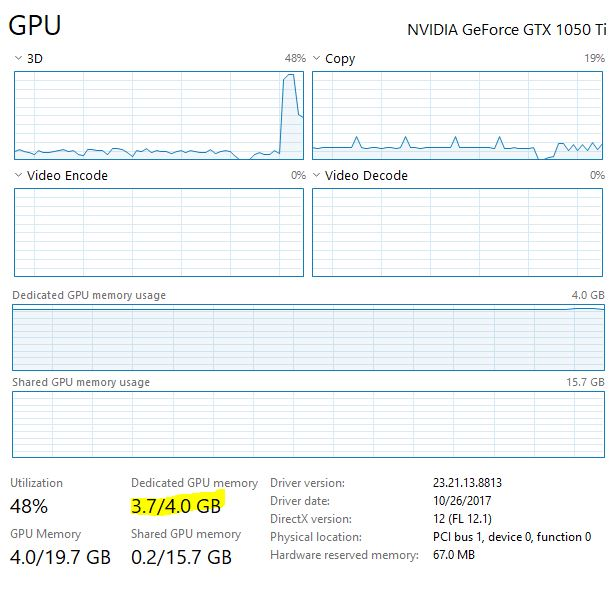
\includegraphics[scale=0.75]{part10-environment.JPG}
    \caption{[Part 10] GPU Environment: NVIDIA GeForce GTX 1050Ti with 4.0GB of GRAM}
    \label{fig:part10}
    \end{center}
\end{figure*}
\clearpage

[Part 10] NN Model
\begin{verbatim}
    def __init__(self, num_classes=1000):
        super(MyAlexNet, self).__init__()
        self.features = nn.Sequential(
            nn.Conv2d(3, 64, kernel_size=11, stride=4, padding=2),
            nn.ReLU(inplace=True),
            nn.MaxPool2d(kernel_size=3, stride=2),
            nn.Conv2d(64, 192, kernel_size=5, padding=2),
            nn.ReLU(inplace=True),
            nn.MaxPool2d(kernel_size=3, stride=2),
            nn.Conv2d(192, 384, kernel_size=3, padding=1),
            nn.ReLU(inplace=True),
            nn.Conv2d(384, 256, kernel_size=3, padding=1),
            nn.ReLU(inplace=True),
            # nn.Conv2d(256, 256, kernel_size=3, padding=1),
            # nn.ReLU(inplace=True),
            nn.MaxPool2d(kernel_size=3, stride=2),
        )
        self.mynet = nn.Sequential(
            nn.Dropout(),
            torch.nn.Linear(256 * 6 * 6, 2048),
            nn.ReLU(inplace=True),
            nn.Dropout(),
            torch.nn.Linear(2048, 12),
            nn.ReLU(inplace=True),
            torch.nn.Linear(12, 6),
        )
    ...
    ...
    def forward(self, x):
        x = self.features(x)
        x = x.view(x.size(0), 256 * 6 * 6)
        x = self.mynet(x)
        return x
    ...
    ...    
    x = Variable(torch.from_numpy(train_x), requires_grad=False).type(dtype_float)
    y_labels = Variable(torch.from_numpy(np.argmax(train_y, 1)),
                requires_grad=False).type(dtype_long)

    myANet = MyAlexNet()
    myANet.cuda()

    loss_fn = torch.nn.CrossEntropyLoss()

    ## TRAINING THE MODEL
    alpha = 1e-2
    optimizer = torch.optim.SGD(myANet.parameters(), lr=alpha, momentum=0.99)

    for t in range(n):
        if t % 50 == 0:
            print('t: ', t)

        # forward
        y_pred = myANet.forward(x)
        ...
        ...
        
\end{verbatim}
In order to get the Conv4 Layer, we commented out the fifth/last convolution layer. Then we apply this layer with our own classification layer (self.mynet(x)) to classify our 6 actors given the labels, whereas the original classification layer will output 1000 kinds of labels for different objects AlexNet has trained with.\\

The detail layers of our newly constructed NN is given above.

\begin{figure*}[h!]
    \begin{center}
    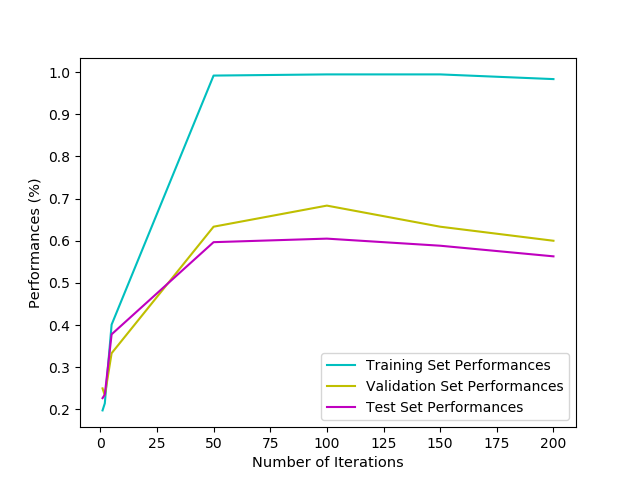
\includegraphics[scale=0.85]{part10-performances-plot.png}
    \caption{[Part 10] Learning Curve}
    \label{fig:part10}
    \end{center}
\end{figure*}
\clearpage


\begin{figure*}[h!]
    \begin{center}
    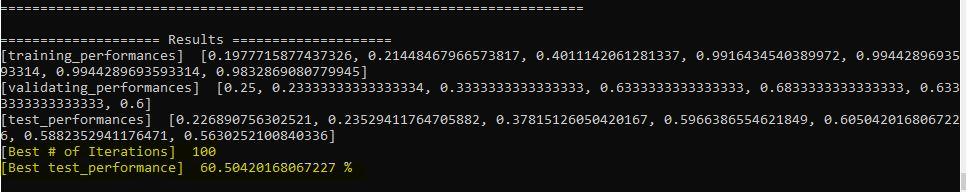
\includegraphics[scale=0.7]{part10-best-result.JPG}
    \caption{[Part 10] Find Best Iteration (max\_iter = 100 from the Learning Curve Figure)}
    \label{fig:part10}
    \end{center}
\end{figure*}

\begin{figure*}[h!]
    \begin{center}
    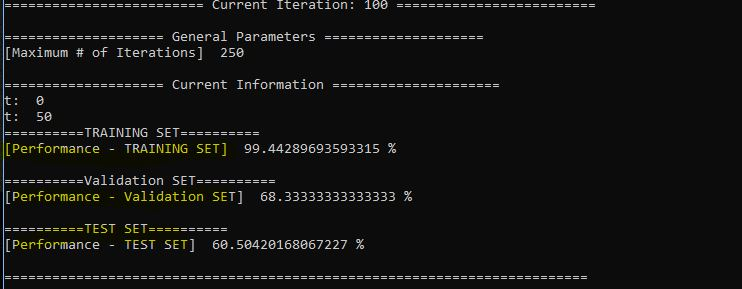
\includegraphics[scale=0.7]{part10-best-result-2.JPG}
    \caption{[Part 10] Use the Best # of Iteration (=100) to get the Performances}
    \label{fig:part10}
    \end{center}
\end{figure*}

From the learning curve, we can see that the best # of iterations we should apply to minimize our cost is using max\_iter = 100, shown in Figure 15.\\
The performance on our test set is 60.58\% while training set is having its performance at almost 100\% (similar to validation set). We can observe that the model is overfitting our training and test datasets.

\end{homeworkProblem}
\clearpage

%----------------------------------------------------------------------------------------

\end{document}